%*******************************************************************************
%****************************** Second Chapter *********************************
%*******************************************************************************
\nomenclature[z-Rpi1]{Rpi0}{Raspberry Pi Zero}
\nomenclature[z-Rpi1]{Rpi}{Raspberry Pi Version 1.0}
\nomenclature[z-Rpi2]{Rpi2}{Raspberry Pi Version 2.0}
\nomenclature[z-Rpi3]{Rpi3}{Raspberry Pi Version 3.0}
\nomenclature[z-CLR]{CLR}{Common Language Runtime}
\nomenclature[z-CL]{CL}{Common Language}
\nomenclature[z-GPU]{GPU}{Graphics Processing unit}
\nomenclature[z-CPU]{CPU}{Central Processing unit}
\nomenclature[z-SOC]{SOC}{System-On-Chip}
\nomenclature[z-GPIO]{GPIO}{General Purpose Input/Output}
\nomenclature[z-ML]{ML}{MetaLanguage, Functional Language}
\nomenclature[z-NPM]{NPM}{Node.js Package Manager}
\nomenclature[z-USB]{USB}{Universal Serial BUS}
\chapter{Preliminari}

\ifpdf
    \graphicspath{{Chapter2/Figs/Raster/}{Chapter2/Figs/PDF/}{Chapter2/Figs/}}
\else
    \graphicspath{{Chapter2/Figs/Vector/}{Chapter2/Figs/}}
\fi


\section{Raspberry Pi}
Il Raspberry Pi è un calcolatore di  dimensioni molto ridotte ed a basso costo realizzato dalla RaspberryPi Fondantion, esistono diversi versioni di questo piccolo computer  così come riportato dalla tabella.

\begin{figure}[htbp!] 
	\centering    
	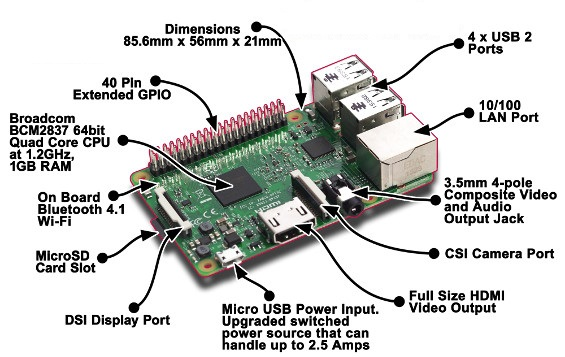
\includegraphics[width=1.0\textwidth]{rpi3}
	\caption[RaspberryPi V3.0]{Raspberry Pi Version 3.0}
	\label{fig:rpi3}
\end{figure}

La scelta per il progetto oggetto di questa tesi è stata per la versione 3  perchè mette a disposizione una potenza di calcolo superiorie a qualunche altro modello di RPi, grazie SoC BCM2837 all'interno del quale c'è  un 1Gb memoria, una CPU un quad-core ARM Cortex A53 a 64 bit a 1.2 Ghz ed una GPU VideoCore IV a 400Mhz, inoltre la Rpi3 è dotata del chip BCM43438 che fornisce connessione Wifi b/g/n e Bluetooth eliminando la necessità di utilizzare  un adatattore Wifi USB come avveniva nelle versioni precedenti.
L'antenna usata per le comunicazioni wireless si  trova sul bordo esterno della scheda, fuori dalla portata di possibili interferenze causate  da eventuali dispositivi e componenti aggiuntivi. L'integrazione delle comunicazioni wireless è una caratteristica importante se si vuole valutare l'aspetto di risparmio economico per una piattaforma IoT.

La Rpi ha quattro porte USB e una porta Ethernet 10/100 che condividono lo stesso bus gestito dal chip LAN9514. Questa soluzione può essere criticata  perchè non permette di sfruttare il 1Gbit sulla porta Ethernet, ma ai fini del nostro progetto non è un difetto che penalizza.


Nel dispositivo non è presente nessun tipo di memoria di massa, ma è presente un lettore di memorie MicroSD.
L'avvio del sistema avviene dalla scheda MicroSD all'interno della quale c'è una partizione con sopra il firmware, kernel e la configurazione del sistema.
Questo calcolatore è stato progettato per funzionare su diversi sistemi operativi Linux, RiscOS e Windows Core Iot.
Nell'appendice A descrivo come installare la versione Linux Raspian, il sistema operativo scelto per questo progetto.

\subsection{GPIO}
Tutte le versioni di questo computer hanno la possabilità di poter utilizzare GPIO  le GPIO sono delle porte che è possibile interagirgi
\begin{figure}[htbp!] 
	\centering    
	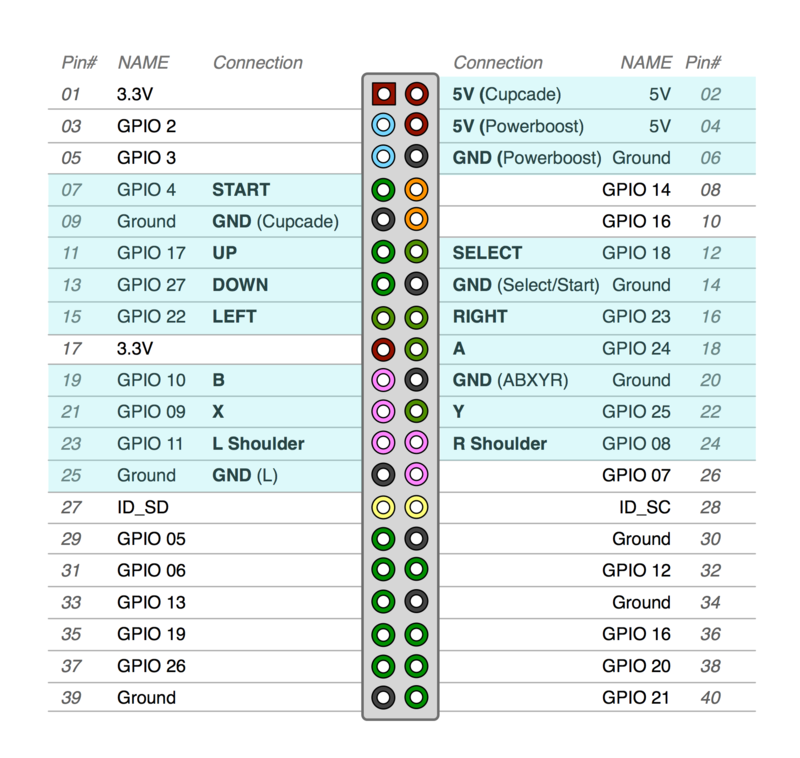
\includegraphics[width=1.0\textwidth]{gpio-map}
	\caption[Mappa GPIO]{La mappa delle Pin GPIO su Raspberry Pi}
	\label{fig:gpio-map}
\end{figure}
Nell'appendice B descrivo un semplice progetto che utilizza le porte GPIO

\subsection{Raspberry Camera}
Questa camera si collega a Raspberry Pi tramite la porta CSI e consente di creare video HD e scattare fotografie digitali,ha integrato il sensore di immagine CMOS IMX219PQ Sony da 8 megapixel ad alta qualità ed elevata sensibilità, con funzioni di video imaging ad alta velocità e supporto delle modalità video 1080p30, 720p60 e VGA90
\begin{figure}[htbp!] 
	\centering    
	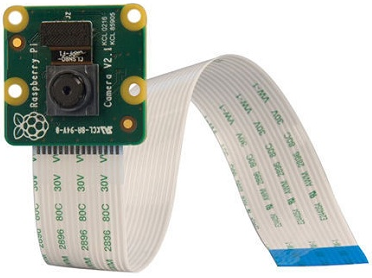
\includegraphics[width=1.0\textwidth]{camera}
	\caption[Raspberry Camera]{La Raspberry Camera}
	\label{fig:camera}
\end{figure}
Nell'appendice B descrivo come utilizzare i comandi offerti da raspian per utilizzare la raspberry camera

\subsection{L298N Motor Controller}
Si tratta di un modulo elettronico basato appunto sull’integrato L298, e sarà utilizzato per pilotare motori.
\begin{figure}[htbp!] 
	\centering    
	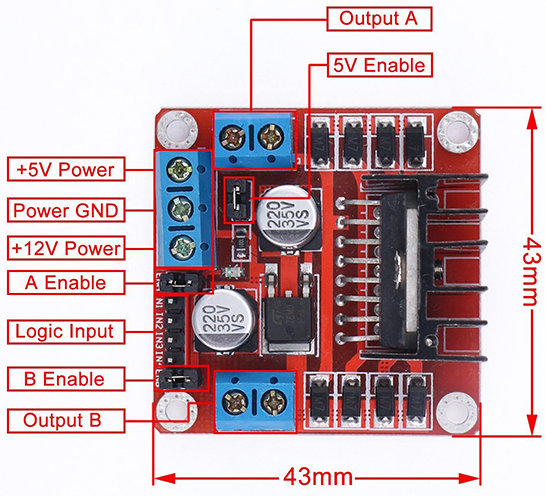
\includegraphics[width=1.0\textwidth]{L298N}
	\caption[L298N Motor Controller]{L298N Motor Controller}
	\label{fig:L298N}
\end{figure}
Questo circuito è composto da due connettori laterali ai quali collegare i motori, e da connettori frontali dove collegare l’alimentazione e le connessioni logiche atte a pilotare i carichi.
\begin{figure}[htbp!] 
	\centering    
	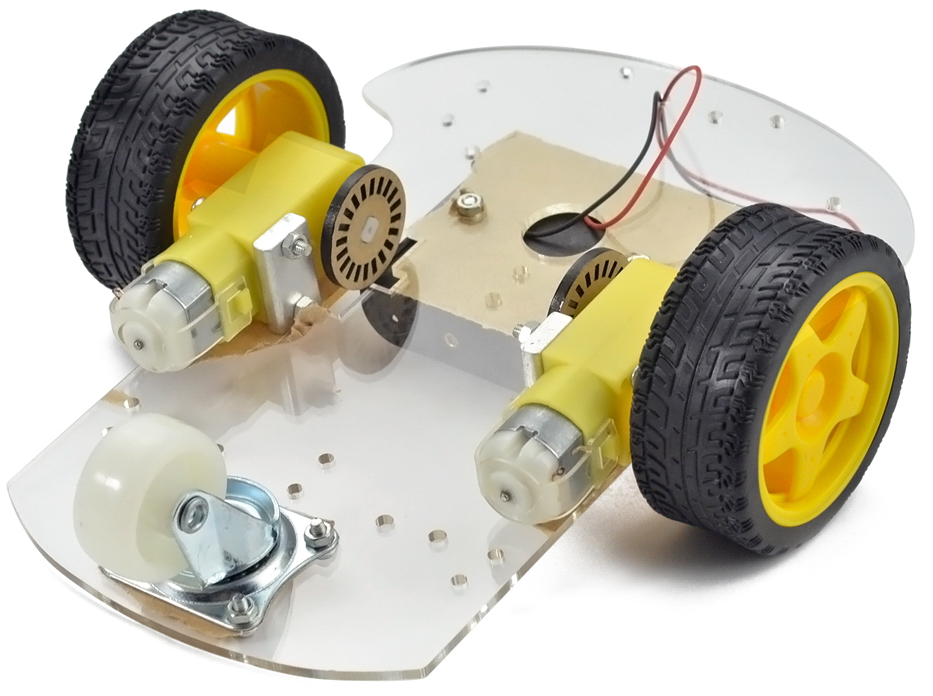
\includegraphics[width=1.0\textwidth]{chassis}
	\caption[Rover Chassis]{Rover Chassis con ruote, vano batteria}
	\label{fig:chassis}
\end{figure}
Questo modulo sarà collegato nel progetto finale direttamente allo chassis dove saranno presenti i motori e il vano batteria


\subsection{HC-SR04}
Il  sensore ad ultrasuoni hc-sr04 emette un impulso ad ultrasuoni e calcola il tempo impiegato dall’impulso per raggiungere il primo ostacolo di fronte a lui e tornare in dietro.
\begin{figure}[htbp!] 
	\centering    
	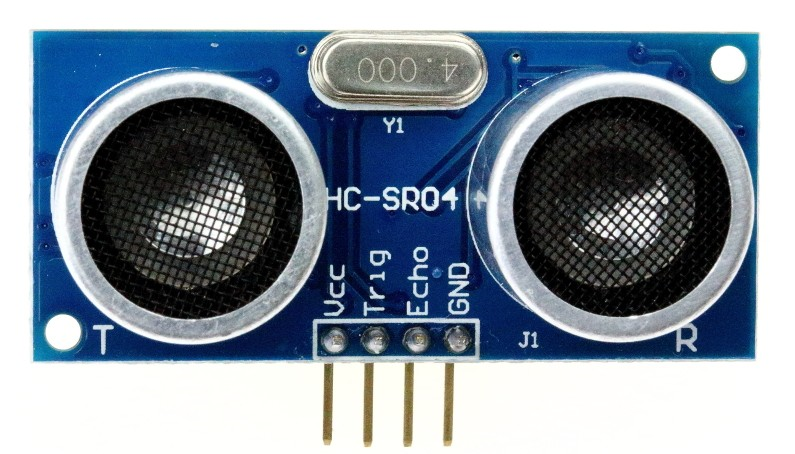
\includegraphics[width=1.0\textwidth]{hc-sr04}
	\caption[HC-SR04]{Il sensore ad ultrasuoni hc-sr04}
	\label{fig:hc-sr04}
\end{figure}
Il sensore dispone di 4 pin: Vcc (+5V), Trigger, Echo, GND. Si invia un impulso alto sul pin Trigger per almeno 10 microsecondi, a questo punto il sensore invierà il ping sonoro e aspetterà il ritorno delle onde riflesse, il sensore risponderà sul pin Echo con un impulso alto della durata corrispondente a quella di viaggio delle onde sonore, dopo 38 millisecondi si considera che non sia stato incontrato alcun ostacolo. Per sicurezza si aspettano in genere 50-60 millisec per far si che non vi siano interferenze con la misura successiva.


\subsection{BreadBoard}
Una breadboard permette di riprodurre il comportamento di un circuito stampato e non richiede saltatura di componenti, è possibile semplicemente inserire i componenti nei fori predisposti sulla board.
\begin{figure}[htbp!] 
	\centering    
	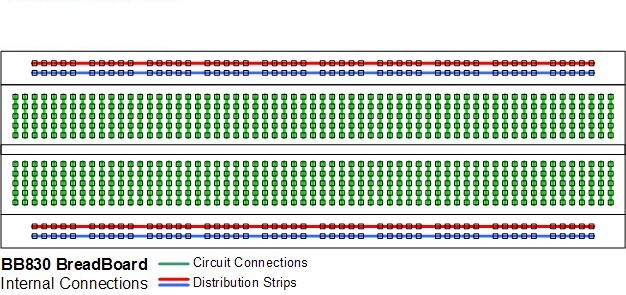
\includegraphics[width=1.0\textwidth]{breadboard}
	\caption[Breadboard]{Breadboard}
	\label{fig:breadboard}
\end{figure}
La breadboard che ho utilizzato è del tipo 830 fori in questo tipo di board ha due linee di punti laterali che corrono per tutta la lunghezza della breadboard e ogni punto di ogni singola linea è collegato tra di loro e solitamente queste linee vengo utilizzate per l’alimentazione. 
Le linee di punti interne della breadboard invece sono collegati a gruppi di due . i gruppi sono divisi da una scanalatura e ognuno dei quali è composto da 5 punti collegati tra loro.
Tutti i punti della breadboard che hanno una distanza di 2.54mm tra loro sono contrassegnati da un numero o da una lettera per facilitarne l'utilizzo.

Per facilitare la costruzione e il testing utilizzero un cavo piatto a 40 pin che collego dal Rpi3 ad un  t-cobbler sopra la breadboard , in questo modo posso lavorare con i GPIO di Rpi3 direttamente sulla board di testing
 

\begin{figure}[htbp!] 
	\centering    
	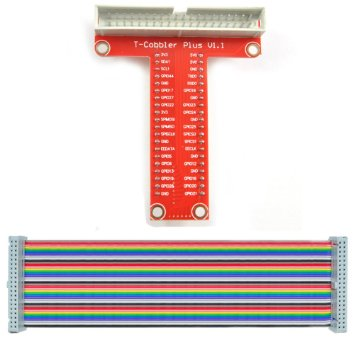
\includegraphics[width=1.0\textwidth]{t-cobbler-40}
	\caption[t-cobbler-40]{Cavo 40 Pin e T-Cobbler}
	\label{fig:t-cobbler-40}
\end{figure}

\section{Mono}
Mono è un progetto opensource coordinato da Xamarin, dal 2015 è diventata un'azienda sussidiaria di Microsoft, che ha lo scopo di realizzare  un insieme di strumenti compatibili con il Framework .NET di Microsoft ed aderenti allo standard Ecma anche per ambienti non Windows.
Il progetto mono implementa sia macchine virtuali chiamata Common Language Runtime per l'esecuzione dei programmi .NET per diverse piattaforme che compilatori per diversi linguaggi di programmazione.

Tra le CLR implementate c'è anche quella per Linux per processori x64 ARM e tra i compilatori di linguaggi implemetanti da Mono c'è sia il compilatore per \texttt{C\#} che quello per \texttt{F\#} che verrano utilizzati in questo progetto.

Nell'appendice C sarà  descritto come installare Mono e il compilatore \texttt{F\#} su Rpi3.

\section{\texttt{Raspberry\# IO}}
Nel progetto utilizzerò Raspberry# IO, è una libreria che consente di utilizzare le funzionalità GPIO di raspberry Pi su ambiente .NET/Mono, questa libreria è utilizzabile su linguaggio F#.
Nello specifico utilizzerò il package Raspberry.IO.GeneralPurpose che consente di utilizzare i Pin GPIO.
Questo package supporta le seguenti caratteristiche
Basso livello:

Accesso ai PIN GPIO attraverso 3 modalità: 
semplice (con uso di file), 
attraverso memoria, e 
completa (memoria attraverso "pseudo-interrupt"). Di default questa è modalità usata.
	Indirizzamento con il numero pin o con il numero di connettore pin
	Assegnamento dei Pin in base al modello e revisione del Raspberry Pi
	uso controllato delle risorse utilizzando un componente IDisposable e la capacità di utilizzare il rilevamento delle soglie , invece di polling
	Supporto al di sotto del millisecondo per il polling dei pin di input

Alto livello:
	Permette di personalizzare il nome dei Pin per consentire una maggiore leggibilità del codice
	Facilità di Uso, configurazione dichiarativa  dei Pin. Possibilità di ripristinare la polarità dei Pin (0/1). Permette di utilizzxare un pin in input come uno switch button.  
	Genera un evento quando lo status di un pin cambia , utlizzando il polling


\section{\texttt{ML}_{CoDa}}
 \texttt{ML}_{CoDa} è un linguaggio di programmazione orientanto al Contesto. Questo linguaggio consente con alcuni costrutti di adattare il programma al contesto in cui viene eseguito. Il prototipo del linguaggio \texttt{ML}_{CoDa} che userò è un estensione del linguaggio funzionale F#, della famiglia dei linguaggi ML.
 
 
 Nell'appendice D descrivo come testare gli esempi di \texttt{ML}_{CoDa} su Mono installato su Rpi3
 Nell'appendice E implemento il progetto button-led in \texttt{ML}_{CoDa} 
\section{Node.js}

Node.js è un ambiente di esecuzione Javascript  opensource ed è disponibile su molte architetture, la piattaforma Node.js è basata sul Javascript Engine V8 di Google.
La principale caratteristica di Node.js è la sua  architettura event-driver per le I/O asincrone.
Inoltre offre anche un sistema di gestione dei pacchetti chiamato npm che permette di  in modo semplice e veloce di scaricare, installare e di integrare nel proprio progetto funzionalità aggiuntive offerte da moduli realizzati da una grandissima comunità.
Nel progetto utilizzero alcuni di questi pacchetti disponibili dal repository ufficale.


\subsection{Express.js}

\subsection{Telegram.js}
L’idea del progetto è di poter interagire con il robot con un I messaggistica, la scelta è caduta su telegram perché consente in maniera semplice di realizzare bot e interagirci attraverso API REST con risultanti in JSON

L'appendice E 

\section{Microsoft Cognitive Services} 
Cognitive Services (anche noto con il nome di Project Oxford) è un insieme di servizi esposti come API REST che permettono di aggiungere alle nostre applicazioni delle funzionalità “cognitive”, cioè funzionalità che abilitano le nostre applicazioni alla “comprensione” del mondo che le circonda.
Cognitive Services sfrutta la potenza del cloud e, in particolar modo, Azure Machine Learning per fornire una pletora di servizi che possiamo dividere nelle seguenti categorie:
•	Vision Service: sono quei servizi che permettono di analizzare immagini o video alla ricerca di informazioni. Fanno parte di questa categoria i servizi che ci consentono di individuare un volto o delle espressioni di un viso o le caratteristiche di un oggetto presente in un’immagine;


